\section{О связности и изоморфизме}

	Изначально я рассчитывал рассказать о связности и изоморфизме в этом параграфе. Эта часть будет ниже, но немного позже. А перед этим будут разобраны небольшое число примеров. Они были добавлены сюда по причине того, что большая часть аудитории, который я читал этот курс, и, возможно, немногочисленная часть читателей не любят останавливаться на прорешивании задач, но при этом были бы непрочь увидеть или услышать решения некоторых задач.

\mysubsection{Компоненты связности}

\begin{definition}
	Вершина $a$ называется \emph{изолированной}, если $deg(a) = 0$.
\end{definition}

\begin{definition}
	Граф, $G(V') = \langle V', E' \rangle$ называется \emph{подграфом}, порожденным множеством вершин $V' \subset V$, если $E'$ содержит только рёбра из $E$, которые соединяют вершины $V'$ между собой.
\end{definition}

\begin{definition}
	\emph{Компонента связности}~---~максимальный связный подграф.
\end{definition}

	Для любителей экзотики и знакомых с понятием эквивалентности можно также добавить, что связность как бинарное отношение есть ни что иное, как отношение эквивалентности, поэтому на самом деле компоненты связности можно определять как классы экивалентности по отношению связности.
	
	Если вы мало поняли, о чём говорится в предыдущем предложении, не расстраивайтесь, когда-нибудь мы ещё вернёмся к этим понятиям и уже более основательно с ними будем работать. 

\begin{statement}
	В лесу на $n$ вершинах с $k$ компонентами связности выполнено равенство
	$$|E| = n - k.$$
	
\begin{proof}
	Возьмём вершину $a$ и проведём из неё $k-1$ ребро в остальные компоненты связности (по одному в каждую). Тогда наш граф эволюционирует в дерево, следовательно, в нём будет $n-1$ ребро. Осталось сделать тривиальные преобразования
	$$|E| = (n-1) - (k-1) = n-k.$$
\end{proof}
\end{statement}
	
\begin{example}
	В некоторой стране 31 город. Известно, что каждый город соединен с не менее чем 15 городами. Докажите, что из любого города можно доехать до любого другого, сделав не более одной пересадки.
	
	\emph{Доказательство.} Построим граф для этой задачи: городами будут вершины, а дороги~---~рёбрами. Допустим, что граф не связен. То есть есть пара городов не соединенных между собой. Тогда в графе, в котором вершины~---~города, а дороги~---~рёбра, будет хотя бы две компоненты связности. Кроме того, в каждой компоненте будет не менее 16 городов. Следовательно, вершин всего будет не менее 32. Противоречие. 
	
	Следовательно, он связен, притом произвольные вершины $a$ и $b$ будут смежными или, как было показано выше, множество смежных вершин дял них будет пересекаться, то есть максимальное расстояние между ними будет равно двум. ч.т.д.
\end{example}
	
\begin{statement}
	Пусть в графе $G$ ровно две вершины имеют нечётную степень. Докажите, что эти вершины являются связанными.
	
	\emph{Доказательство.} Допустим, что $a$ и $b$~---~две вершины с нечётной степенью, несвязанны. Тогда в компоненте связности, в которой лежит вершина $a$ нечётных вершин только одна, так как по условию все остальные вершины будут чётной степени. Это противоречит лемме о рукопожатиях. Следовательно, $a$ и $b$ связаны. ч.т.д.
\end{statement}

\mysubsection{Мост и точка сочленения}

	В математике полезно изучать не только какие-то <<полные классы>> графов, но и некоторые полуклассы, то есть такие наборы объектов, каждый из которых можно получить путём изменения незначительно какого-нибудь параметра для объекта <<полного класса>>. В этом случае, например, есть графы, которые при удалении ребра или вершины теряют свою связность. С ними связаны следующие определения.

\begin{definition}
	Ребро $e \in E$ связного графа $G(V, E)$ называется \emph{мостом}, если после его удаления граф становится несвязным. Граф, полученный при удалении ребра $e$ из графа $G$, обычно обозначается $G - e$.
\end{definition}

\begin{definition}
	Вершина $a$ называется \emph{точкой сочленения} графа $G$, если после её удаления число компонент связности увеличивается по сравнению с числом компонент связности исходного графа. Граф, полученный при удалении вершины $a$ из графа $G$, обычно обозначается $G - a$.
\end{definition}

	Далее разберём критерии моста и точки сочленения.
	
\begin{statement}
	Вершина $a$ является точкой сочленения графа $G$, построенного на $n \geqslant 3$ вершинах, тогда и только тогда, когда в $G$ существует такие отличные от $a$ вершины $b$ и $c$, что любой путь, соединяющий их, проходит через $a$.
	
	\emph{Доказательство.} Условие эквивалентно тому, что после удаления вершины $a$, две другие вершины станут несвязанными. Утверждение становится очевидным. ч.т.д.
\end{statement}

\begin{statement}
	Ребро $e = \left\lbrace a, b \right\rbrace$ в простом связном графе является мостом тогда и только тогда, когда $e$ не принадлежит ни одному из циклов графа.
	
	\emph{Доказательство.} Докажем в обратную сторону. Допутим противное. Тогда в графе $G - e$ будет одна компонента связности и вершины $a$ и $b$ будут связанными путём~$P$. Этот путь вместе с ребром $e$ будет порождать цикл. Противоречие.
	
	В прямую сторону доказательство аналогично. ч.т.д.
\end{statement}

\mysubsection{Изоморфизм графов}

	А сейчас пора сказать о некоторой обманке: мы до этого говорили, что можно <<передвигать>> вершины и растягивать, сжимать рёбра. На самом деле в этом случае мы основывались на том, что изоморфные графы не различаются между собой в теории графов. Объясним, что такое изоморфизм.

\begin{definition}
Графы $G_1$ и $G_2$ \emph{изоморфны}, если можно пронумеровать вершины обоих графов так, чтобы при наличии ребра, соединяющего вершины $i$ и $j$ в одном из графов, в другом было такое же ребро. Если в одном из графов есть петля, выходящая и входящая в вершину $s$, то и в другом должна быть петля при вершине~$s$. Кратность ребер тоже сохраняется.
\end{definition}

	Для знатоков также можно добавить, что графы изоморфны тогда и только тогда, когда существует взаимнооднозначное соответствие между вершинами такое, что сохраняется отношение смежности.

	Чтобы понять, что такое изоморфные графы, можно представить, что вершины~---~это узлы, а ребра~---~очень эластичные нитки. А изоморфны те графы, которые можно наложить друг на друга, растягивая и сжимая эти нитки.

\begin{center}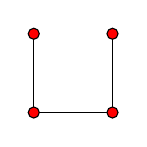
\begin{tikzpicture}
	\tikzstyle{every node}=[circle, draw, fill=red, inner sep=0pt, minimum width=4pt]
	
	\draw (0, 1) -- (0, 0) -- (1, 0) -- (1, 1);
    
    \draw (0, 1) node {}
    	  (0, 0) node {}
    	  (1, 0) node {}
    	  (1, 1) node {};
\end{tikzpicture} \;\ \;\ 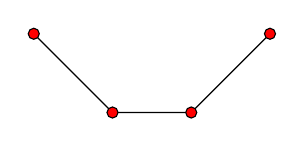
\begin{tikzpicture}
	\tikzstyle{every node}=[circle, draw, fill=red, inner sep=0pt, minimum width=4pt]
	
	\draw (-1, 1) -- (0, 0) -- (1, 0) -- (2, 1);
    
    \draw (-1, 1) node {}
    	  (0, 0) node {}
    	  (1, 0) node {}
    	  (2, 1) node {};
\end{tikzpicture} \;\ \;\ 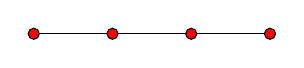
\begin{tikzpicture}
	\tikzstyle{every node}=[circle, draw, fill=red, inner sep=0pt, minimum width=4pt]
	
	\draw (-1, 0) -- (0, 0) -- (1, 0) -- (2, 0);
    
    \draw (-1, 0) node {}
    	  (0, 0) node {}
    	  (1, 0) node {}
    	  (2, 0) node {};
\end{tikzpicture} \;\ \;\ 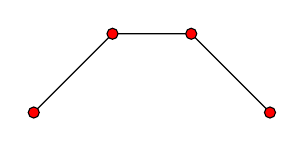
\begin{tikzpicture}
	\tikzstyle{every node}=[circle, draw, fill=red, inner sep=0pt, minimum width=4pt]
	
	\draw (-1, -1) -- (0, 0) -- (1, 0) -- (2, -1);
    
    \draw (-1, -1) node {}
    	  (0, 0) node {}
    	  (1, 0) node {}
    	  (2, -1) node {};
\end{tikzpicture} \;\ \;\ 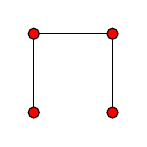
\begin{tikzpicture}
	\tikzstyle{every node}=[circle, draw, fill=red, inner sep=0pt, minimum width=4pt]
	
	\draw (0, -1) -- (0, 0) -- (1, 0) -- (1, -1);
    
    \draw (0, -1) node {}
    	  (0, 0) node {}
    	  (1, 0) node {}
    	  (1, -1) node {};
\end{tikzpicture}
\newline
\newline
	\small Рис. 23. Пять изоморфных графов
\end{center}
	
\begin{statement}
	В изоморфных графах одинаковое количество компонент связностей.
	
	\emph{Доказательство.} Заметим, что если какие-либо две вершины соединены путем в одном из этих графов, то и в другом они тоже будут соединены, поэтому связность вершин инварианта относительно изоморфизма.
\end{statement}

	Говоря о неизоморфных графах, принято называть их \emph{непомеченными}. В свою очередь, когда мы различаем изоморфные графы, построенные на одних и тех же вершинах, то будем их называть \emph{помеченными}.


\begin{statement}
	Графы $G$ и $H$ изоморфны тогда и только тогда, когда изоморфны их дополнения $\overline{G}$ и $\overline{H}$.
	
	\emph{Доказательство.} Заметим, что изоморфизм сохраняет также отношение несмежности, которое эквивалентно отношению смежности вершин в дополнении к графу. Таким образом, изоморфизм графов $G$ и $H$ сохраняет отношение смежности между их дополнениями, следовательно, $\overline{G}$ и $\overline{H}$ изоморфны. А также воспользуемся свойством дополнения, а именно, тем, что дополнение к дополнению графа~---~это сам граф. Таким образом, доказанное утверждение верно в обе стороны. ч.т.д.
\end{statement}
$ $
\newline
	В этом параграфе мы наконец сформулировали, какие графы мы считаем одинаковыми. На самом деле изоморфизм имеет более широкое значение в высшей алгебре, так что с этим понятием читатель ещё не раз встретится на пути изучения математики. А о связности графов мы ещё будем дальше говорить, но уже в терминах орграфов.

\newpage
\mysubsection{Задачи}

\begin{exersize}
	При каких $n$ число неизоморфных попарно деревьев на $n$ вершинах будет равно $n$?
\end{exersize} 

\begin{exersize}
	Нарисуйте три неизоморфных графа со степенной последовательностью (3, 3, 2, 2, 1, 1).
\end{exersize}

\begin{exersize}
	В группе из нескольких человек некоторые люди знакомы друг с другом, а некоторые нет. Каждый вечер один из них устраивает ужин для всех своих знакомых, на котором знакомит их друг с другом. После того, как каждый человек устроил хотя бы по одному ужину, оказалось, что какие-то два человека все еще не знакомы. Докажите, что они не познакомятся и на следующем ужине.
\end{exersize}

\begin{exersize}
	Докажите, что простой граф $G$, минимальная степень $\delta (G)$ которого не меньше $\frac{n}{2}$, является связным. Покажите, что эта оценка точная, предъявив несвязный граф, для которого $\delta (G) = \frac{n}{2} - 1$.
\end{exersize}

\begin{exersize}
	Пусть $G$~---~граф, имеющий $k$ компонент связности, построенный на $n$ вершинах. Докажите, что для количества рёбер имеет место два неравенства $$n-k \leqslant m \leqslant \frac{(n-k)(n-k+1)}{2}.$$
\end{exersize}

\begin{exersize}
	Верно ли, что при любом натуральном $k$, если в графе ровно $4k$ вершин имеют степень 5, а степени остальных~---~6, то нельзя удалить одно ребро так, чтобы этот граф распался на две изоморфные компоненты связности?
\end{exersize}

\begin{exersize}
	Удаленностью вершины дерева назовём сумму расстояний от неё до всех остальных вершин. Докажите, что в дереве, у которого есть две вершины с удаленностями, отличающимичся на 1,~---~нечётное число вершин.
\end{exersize}	

\begin{exersize}
	Докажите, что в любом графе $G$ для расстояния $d(a, b)$ выполняется неравенство треугольника, то есть 
	$$d(a, b) + d(b, c) \leqslant d(a,c) \;\ \forall \!\ a, b, c \in V.$$
\end{exersize}	

\begin{exersize}
	Пусть $G$~---~произвольный простой несвязный граф. Докажите, что его дополнение $\overline{G}$ всегда связно.
\end{exersize}	

\begin{exersize}
	Пусть в графе $G$ $45$ вершин и степень каждой из них не меньше 22. Докажите, что любые две вершины $a$ и $b$ графа $G$ либо смежны, либо $d (a, b) = 2$. 
\end{exersize}	

\begin{exersize}
	Сколько рёбер должен иметь простой граф на $n$ вершинах, чтобы он был гарантированно связным?
\end{exersize}

\begin{exersize}
	Докажите, что если в графе $G$ больше одной компоненты связности, то его дополнение $\overline{G}$ связно.
\end{exersize}

\begin{exersize}
	Граф $G$ называется самодополнением (self-complementary), если он изоморфен своему дополнению $\overline{G}$. Приведите примеры самодополненных графов, построенных на четырёх и пяти вершинах.
\end{exersize}

\begin{exersize}
	Докажите, что любое ребро дерева~---~мост и любая вершина, которая не является листом,~---~это точка сочленения.
\end{exersize}

\begin{exersize}
	В стране Роботлэнд каждый город соединен ровно с 2018 другими, причём из любого города можно добраться до любого другого. Докажите, что после проливных дождей, затопивших одну из дорог, всё ещё можно будет добраться из любого города до любого другого.
\end{exersize}

\begin{exersize}
	Пусть $G$~---~граф, построенный на вершинах $1, 2, \dots, 15$, в котором вершины $i$ и $j$ смежны тогда и только тогда, когда их наибольший общий делитель больше единицы. Подсчитайте число связных компонент такого графа, а также определите максимальную длину простого пути в графе $G$.
\end{exersize}

\begin{exersize}(Канель-Белов А.Я., Ковальджи А.К. Как решают нестандартные задачи)
	В спортклубе тренируются $100$ толстяков, веса которых равны $1$ кг, $2$ кг, ..., $100$ кг. На какое наименьшее число команд их можно разделить, чтобы ни в какой командене было двух толстяков, оидн из которых вдвое тяжелее другого?
\end{exersize}

\begin{exersize}[Канель-Белов А.Я., Ковальджи А.К. Как решают нестандартные задачи]
	В стране больше $101$ города. Столица соединена с $100$ городами, а каждый город, кроме столицы, соединен авиалиниями ровно с $10$ городами (есил $A$ соединен с $B$, то $B$ соединен с $A$). Известно, что из любого города можно попасть в любой другой (быть может, с пересадками). Докажите, что можно закрыть половину авиалиний, идущих из столицы, так, что возможность попасть из любого города в любой другой сохранится.
\end{exersize}

\begin{exersize}[Бабичева Т.С., Бабичев С.Л., Жогов А. А., Яковлев И.В. <<Пособие по олимпиадной математике. Уровень А1>>]
	В Империи Вестероса было $1000$ городов и $2017$ дорог (каждая дорога соединяет какие-то два города). Из каждого города можно было проехать в каждый. Однажды злой волшебник заколдовал $N$ дорог, и ездить по ним стало нельзя. Образовалось $7$ королевств, так, что в каждом королевстве можно добраться из любого города в любой по дорогам, а из одного королевства в другое по дорогам добраться нельзя. При каком наибольшем $N$ это возможно?
\end{exersize}

\begin{exersize}[Агаханов Н.Х., Богданов И.И., Кожевников П.А., Подлипский О.К., Терешин Д.А. <<Всероссийские олимпиады школьников по математике 1993~---~2009: Заключительные этапы>>]
	Внутри круга расположены точки $A_1, A_2, \dots, A_n$, а на его границе~---~точки $B_1, B_2, \dots, B_n$ так, что отрезки $A_1B_1, A_2B_2, \dots, A_nB_n$ не пересекаются. Кузнечик может перепрыгнуть из точки $A_i$ в точку $A_j$, если отрезок $A_iA_j$ не пересекается ни с одним из отрезков $A_kB_k, k \neq i, j$. Докажите, что за несколько прыжков кузнечик сможет попасть из любой точки $A_p$ в любую точку $A_q$.
\end{exersize}	

\begin{exersize}[Агаханов Н.Х., Богданов И.И., Кожевников П.А., Подлипский О.К., Терешин Д.А. <<Всероссийские олимпиады школьников по математике 1993~---~2009: Заключительные этапы>>]
	В стране $N$ $1988$ городов и из каждого осуществляются беспосадочные перелеты в три других города (все авиарейсы двусторонние). Известно, что из любого города, сделав несколько пересадок, можно долететь до любого другого. Министр Безопасности хочет объявить закрытыми $200$ городов, никакие два из которых не соединены авиалинией. Докажите, что это можно сделать так, чтобы можно было долететь из любого незакрытого города в любой другой, не делая пересадок в закрытых городах.
\end{exersize}	 

\begin{exersize}[Агаханов Н.Х., Богданов И.И., Кожевников П.А., Подлипский О.К., Терешин Д.А. <<Всероссийские олимпиады школьников по математике 1993~---~2009: Заключительные этапы>>]
	В стране несколько городов, некоторые пары городов соединены беспосадочными рейсами одной из $N$ авиакомпаний, причем из каждого города есть ровно по одному рейсу каждой из авиакомпаний. Известно, что из любого города можно долететь до любого другого (возможно, с пересадками). Из-за финансового кризиса был закрыт $N-1$ рейс, но ни в одной из авиакомпаний не закрыли более одного рейса. Докажите, что по-прежнему из любого города можно долететь до любого другого.
\end{exersize}	 

\begin{exersize}[Агаханов Н.Х., Богданов И.И., Кожевников П.А., Подлипский О.К., Терешин Д.А. <<Всероссийские олимпиады школьников по математике 1993~---~2009: Заключительные этапы>>]
	В некоторой стране $2002$ города, соединенных дорогами так, что если запретить проезд через любой из городов, то из любого из оставшихся городов можно добраться до любого другого. Каждый год король выбирает некоторый несамопересекающийся циклический маршрут и приказывает построить новый город, соединить его дорогами со всеми городами выбранного маршрута, а все дороги этого маршрута закрыть за ненадобностью. Через несколько лет в стране не осталось ни одного несамопересекающегося циклического маршрута, проходящего по ее городам. Докажите, что в этот момент количество городов, из которых выходит ровно одна дорога, не меньше $2002$.
\end{exersize}	 

\begin{exersize}[Агаханов Н.Х., Богданов И.И., Кожевников П.А., Подлипский О.К., Терешин Д.А. <<Всероссийские олимпиады школьников по математике 1993~---~2009: Заключительные этапы>>]
	Множество клеток на клетчатой плоскости назовем \emph{ладейно связным}, если из любой его клетки можно попасть в любую другую, двигаясь по клеткам этого множества ходом ладьи (ладье разрешается перелетать через поля, не принадлежащие нашему множеству). Докажите, что ладейно связаное множество из $100$ клеток можно разбить на пары клеток ,лежащих в одной строке или в одном столбце.
\end{exersize}	

\begin{exersize}[Федоров Р. М., Канель-Белов А. Я., Ковальджи А. К., Ященко И. В. <<Московские математические олимпиады>>]
	В стране Нашии есть военные базы, моединенные дорогами. Набор дорог называется \emph{важным}, если после закрытия этих дорог найдутся две базы, не соединенные путем. Важный набор называется \emph{стратегическим}, если он не содержит меньшего важного набора. Докажите, что множество дорог, каждая из которых принадлежит ровно одному из двух различных стратегических наборов, образует важный набор.
\end{exersize}	